\subsection{Taggre : un cadriciel pour agréger des tâches}
Nous avons pour but de garder la façon naturelle de décrire le parallélisme dans les noyaux d'algèbre linéaire creuse.
%
Malheureusement, cette granularité est trop fine, l'ordonnanceur de tâches met plus de temps à choisir quel sera le processeur qui traitera la tâche que le processeur à traiter la tâche.
%
Pour obtenir des performances raisonnables, nous devons augmenter la granularité de la description du problème.
%
Pour cela, nous proposons de créer des groupes de tâches, de considérer chaque groupe comme une seule tâche et d'ordonnancer tous ces groupes en tant que graphe de tâches pour ainsi réduire le surcoût lié à l'ordonnanceur.
%
Au final, nous obtenons un graphe composé de moins de tâches, mais il faut faire attention à ne pas trop réduire le parallélisme fourni par le graphe.


En partant de la représentation la plus fine sous forme de DAG du parallélisme, nous avons besoin de calculer un nouveau DAG plus grossier avec moins de tâches.
%
La principale difficulté est de garder la propriété {\em acyclique} du graphe, la présence d'un cycle introduirait un inter-blocage dans l'ordonnancement du graphe (Fig.~\ref{fig:agg_invalid}).
%
L'autre difficulté est de maintenir assez de parallélisme pour pouvoir être capable d'utiliser au mieux les capacités de la machine.

\begin{figure}[!ht]
     \begin{center}
        \subfigure[Agrégation invalide]{%
          \label{fig:agg_invalid}
          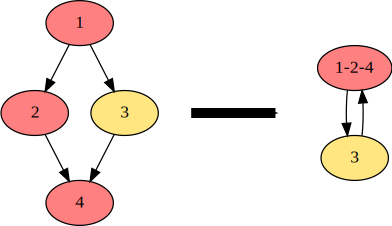
\includegraphics[width=0.4\textwidth]{agg_invalid}
        }%
        \hspace{0.15\textwidth}%
        \subfigure[Agrégation valide]{%
          \label{fig:agg_valid}
          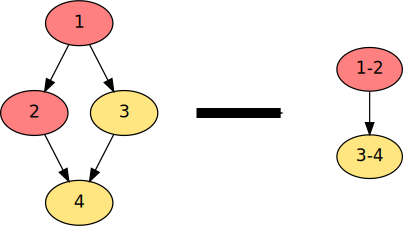
\includegraphics[width=0.4\textwidth]{agg_valid}
        }%
    \end{center}
    \caption{Exemple de deux agrégations, le résultat de \ref{fig:agg_invalid} ne peut pas être ordonnancé à cause du cycle. Le résultat de \ref{fig:agg_valid} peut être ordonnancé mais il n'y a aucun parallélisme à exploiter.}
    \label{fig:agg_basic}
\end{figure}

En premier lieu, nous avons développé une nouvelle interface de programmation basée sur celle de Intel TBB.
%
Cette interface nous permet de décrire un graphe de tâche complet et d'utiliser plusieurs ordonnanceurs pour ordonnancer le graphe.
%
Avec cette interface, nous pouvons faire des modifications sur le graphe et le rendre plus grossier.
%
Nous avons appelé cette interface Taggre.
%
Grâce à l'utilisation d'heuristiques décrites plus loin dans la thèse, un programme parallèle peut continuer de décrire son parallélisme de façon naturelle, sans se soucier de la granularité.
%
Taggre s'occupera ensuite de faire le travail nécessaire pour rendre ce graphe assez grossier pour qu'un ordonnanceur puisse l'ordonnancer efficacement (Fig.~\ref{fig:coarsening}).

%   (-_-)   %
\begin{figure}[t!]
  \centering
  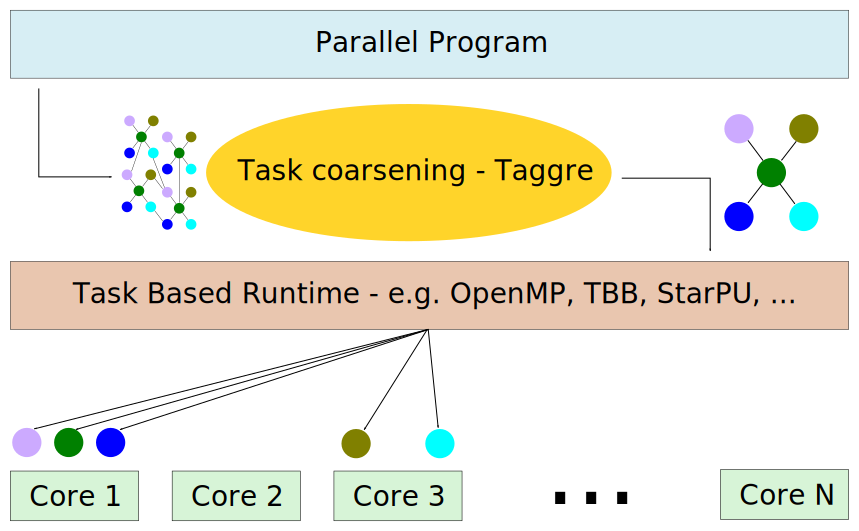
\includegraphics[width=0.8\textwidth]{coarsening}
  \caption{Le programme parallèle fournit un graphe de tâches à Taggre. Taggre modifie le graphe. Taggre fournit le graphe à l'ordonnanceur. Le processus d'agrégation est totalement transparent pour l'ordonnanceur.}
  \label{fig:coarsening}
\end{figure}
